\section{Медиана и порядковые статистики. Алгоритм с линейным временем работы для медианы}

\textbf{k-я порядковая статистика} набора элементов линейно упорядоченного множества --- такой его элемент, который является k-м элементом набора в порядке сортировки

\textbf{Медиана} --- k-я порядковая статистика при $k = N/2$ (если $N$ не кратно двум, то будем рассматривать нижнюю медиану $k = \lfloor N/2 \rfloor$ и верхнюю медиану $k = \lceil N/2 \rceil$

\textbf{Алгоритм с линейным временем работы}
Идея алгоритма напоминает QuickSort.

Сам алгоритм:
\begin{enumerate}
	\item Все n элементов входного массива разбиваются на группы по пять элементов, в последней группе будет $n \: \text{mod} \: 5$ элементов. 
	Эта группа может оказаться пустой при $n$ кратным 5.
	\item Сначала сортируется каждая группа, затем из каждой группы выбирается медиана.
	\item Путем рекурсивного вызова шага определяется медиана $x$ из множества медиан (верхняя медиана в случае чётного количества), найденных на втором шаге. Найденный элемент массива $x$ используется как рассекающий (за $i$ обозначим его индекс).
	\item Массив делится относительно рассекающего элемента $x$.
	\item Если $i=k$, то возвращается значение $x$. Иначе запускается рекурсивно поиск элемента в одной из частей массива: $k$-ой статистики в левой части при $i>k$ или $(k-i-1)$-ой статистики в правой части при $i<k$
\end{enumerate}

\textbf{Доказательство оценки сложности:}

Cначала определим нижнюю границу для количества элементов, превышающих по величине рассекающий элемент x. В общем случае как минимум половина медиан, найденных на втором шаге, больше или равны медианы медиан x. Таким образом, как минимум $\frac{n}{10}$ групп содержат по 3 превышающих величину x, за исключение группы, в которой меньше 5
элементов и ещё одной группы, содержащей сам элемент x. Таким образом получаем, что количество элементов больших x, не менее $\frac{3n}{10}$.

Проведя аналогичные рассуждения для элементов, которые меньше по величине, чем рассекающий элемент x, мы получим, что как минимум $\frac{3n}{10}$
меньше, чем элемент x.

\begin{figure}[ht!]
	\centering
	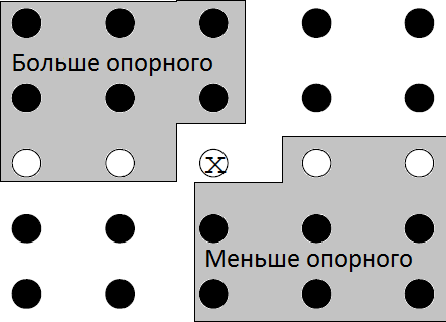
\includegraphics[width=0.7\linewidth]{img_easy/1_1.png}
	\captionsetup{labelformat=empty}
	\caption{Иллюстрация к рассуждению выше}
\end{figure}

Само время работы $T(n)$ не меньше, чем
\begin{enumerate}
	\item Время работы на сортировку группы (одна группа сортируется за константное время, так как в каждой группе константное количество элементов) и разбиение по рассекающему элементу (аналогично операции merge) --- $O(n)$
	\item времени работы для поиска медианы медиан, то есть $T\left(\frac{n}{5}\right)$
	\item времени работы для поиска $k$-го элемента в одной из двух частей массива, то есть $T(s)$, где s --- количество элементов в этой части. Но s
	не превосходит $\frac{7n}{10}$, так как чисел, меньших рассекающего элемента, не менее $\frac{3n}{10}$ --- это $\frac{n}{10}$
	медиан, меньших медианы медиан, плюс не менее 2n10
	элементов, меньших этих медиан. С другой стороны, чисел, больших рассекающего элемента, так же не менее $\frac{3n}{10}$, следовательно, $s \leq \frac{7n}{10}$, то есть в худшем случае $s=
	\frac{7n}{10}$.
\end{enumerate}

Итоговое время работы:
\[
	T(n) \leq T\left(\frac{7n}{10}\right) + T\left(\frac{n}{5}\right) + Cn
\]

Докажем по индукции, что $T(n) \leq 10Cn$

Предположим, что наше неравенство $T(n) \leq 10Cn$ выполняется при малых $n$, для некоторой достаточно большой константы $C$. 
Тогда, по предположению индукции, 

$$
T(n) \leq T\left(\frac{7n}{10}\right) + T\left(\frac{n}{5}\right) + Cn \leq 10C \cdot \frac{7n}{10} + 10C \cdot \frac{n}{5} + Cn = 10 Cn
$$
Значит, итоговая сложность алгоритма $O(n)$